\documentclass[../mathNotesPreamble]{subfiles}
\begin{document}
%\relscale{1.4} %TODO
\section{15.6: Tangent Planes and Linear Approximation}

  \begin{defn*}[Equation of the Tangent Plane for $F(x,y,z)=0$]
    Let $F$ be differentiable at the point $P_0(a,b,c)$ with $\grad F(a,b,c)\neq \bfO$. The plane tangent to the surface $F(x,y,z)=0$ at $P_0$, called the \textbf{tangent plane}, is the plane passing through $P_0$ orthogonal to $\grad F(a,b,c)$. An equation of the tangent plane is
      \[F_x(a,b,c)(x-a)+F_y(a,b,c)(y-b)+F_z(a,b,c)(z-c)=0\]
  \end{defn*}

  \begin{ex*}
    Consider the ellipsoid 
      \[F(x,y,z)= \frac{x^2}{9}+\frac{y^2}{25}+z^2-1=0.\]
    \begin{tasks}[after-item-skip=\stretch{1}](1)
      \task Find an equation of the plane tangent to the ellipsoid at $(0,4, \frac{3}{5})$.
      \task At what points on the ellipsoid is the tangent plane horizontal?
    \end{tasks}
  \end{ex*}
  \vspace*{\stretch{1}}
  \pagebreak

  \noindent
  Surfaces of the form $z=f(x,y)$ are a special case of $F(x,y,z)=0$:\newline Define $F(x,y,z)=z-f(x,y)=0$, then
    \[\grad F\parens{a,b,f(a,b)}=\bracket{-f_x(a,b),\,-f_y(a,b),\,1}\]
  so the tangent plane is
    \[-f_x(a,b)(x-a)-f_y(a,b)(y-b)+1\parens{z-f(a,b)}=0\]
  \begin{thmBox*}[Tangent Plane for $z=f(x,y)$]
    Let $f$ be differentiable at the point $(a,b)$. An equation of the plane tangent to the surface $z=f(x,y)$ at the point $(a,b,f(a,b))$ is
      \[z=f_x(a,b)(x-a)+f_y(a,b)(y-b)+f(a,b)\]
  \end{thmBox*}

  \begin{ex*}
    Find an equation of the plane tangent to $f(x,y)=4e^{xy^2}$ at $(3,0,4)$ and $(0,2,4)$.
  \end{ex*}
  \vspace*{\stretch{1}}
  \pagebreak

  \begin{ex*}
    Find an equation of the plane tangent to $f(x,y)=\tan\inv(xy)$ at $\parens{\sqrt{3},\,1,\,\frac{\pi}{3}}$ and $\parens{\frac{\sqrt{3}}{3},1,\frac{\pi}{6}}$.
  \end{ex*}
  \vspace*{\stretch{1}}

  \begin{defn*}[Linear Approximation]
    Let $f$ be differentiable at $(a,b)$. The linear approximation to the surface $z=f(x,y)$ at the point $(a,b,f(a,b))$ is the tangent plane at that point, given by the equation
      \[L(x,y)=f_x(a,b)(x-a)+f_y(a,b)(y-b)+f(a,b),\]
    For a function of three variables, the linear approximation to $w=f(x,y,z)$ at the point $(a,b,c,f(a,b,c))$ is given by
      \[L(x,y,z)=f_x(a,b,c)(x-a)+f_y(a,b,c)(y-b)+f_z(a,b,c)(z-c)+f(a,b,c).\]
  \end{defn*}
  \pagebreak

  \begin{ex*}
    Let $f(x,y)=\ds\frac{5}{x^2+y^2}$. Find the linear approximation to the function at the point $(-1,2,1)$. Use this to approximate $f(-1.05, 2.1)$.
  \end{ex*}
  \vspace*{\stretch{1}}
  
  \begin{ex*}
    Let $f(x,y)=\sqrt{x^2+y^2}$. Find the linear approximation to the function at the point $(-8,15,17)$. Use this to approximate $f(-7.91, 14.96)$.
  \end{ex*}
  \vspace*{\stretch{1}}
  \pagebreak

  \begin{defn*}[The differential $dz$]
    Let $f$ be differentiable at the point $(x,y)$. The change in $z=f(x,y)$ as the independent variables change from $(x,y)$ to $(x+dx, y+dy)$ is denoted $\Delta z$ and is approximated by the differential $dz$:
      \[\Delta z\approx dz= f_x(x,y)\,dx+f_y(x,y)\,dy.\]
  \end{defn*}

  \begin{ex*}
    Let $z=f(x,y)=\ds\frac{5}{x^2+y^2}$. Approximate the change in $z$ when the variables change from $(-1,2)$ to $(-0.93, 1.94)$.
  \end{ex*}
  \vspace*{\stretch{1}}
  \pagebreak

  \begin{minipage}{0.775\linewidth}
    \begin{ex*}
      A company manufactures cylindrical aluminum tubes to rigid specifications. The tubes are designed to have an outside radius of $r=10\ cm$, a height of $h=50\ cm$, and a thickness of $t=0.1\ cm$. The manufacturing process produces tubes with a maximum error of $\pm0.05\ cm$ in the radius and height, and a maximum error of $\pm 0.0005\ cm$ in the thickness. The volume of the cylindrical tube is $V(r,h,t)=\pi ht(2r-t)$. Use differentials to estimate the maximum error in the volume of a tube.
    \end{ex*}
  \end{minipage}%
  \begin{minipage}{0.225\linewidth}
    \begin{flushright}
      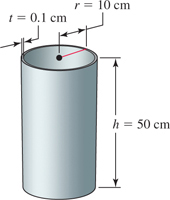
\includegraphics[width=0.9\linewidth]{../images/briggs_15_06/fig15_66}
    \end{flushright}
  \end{minipage}
  \vspace{\stretch{1}}
  \pagebreak

  
\end{document}
